\documentclass[]{article}
\usepackage{lmodern}
\usepackage{amssymb,amsmath}
\usepackage{ifxetex,ifluatex}
\usepackage{fixltx2e} % provides \textsubscript
\ifnum 0\ifxetex 1\fi\ifluatex 1\fi=0 % if pdftex
  \usepackage[T1]{fontenc}
  \usepackage[utf8]{inputenc}
\else % if luatex or xelatex
  \ifxetex
    \usepackage{mathspec}
  \else
    \usepackage{fontspec}
  \fi
  \defaultfontfeatures{Ligatures=TeX,Scale=MatchLowercase}
\fi
% use upquote if available, for straight quotes in verbatim environments
\IfFileExists{upquote.sty}{\usepackage{upquote}}{}
% use microtype if available
\IfFileExists{microtype.sty}{%
\usepackage{microtype}
\UseMicrotypeSet[protrusion]{basicmath} % disable protrusion for tt fonts
}{}
\usepackage[margin=1in]{geometry}
\usepackage{hyperref}
\hypersetup{unicode=true,
            pdftitle={Engsci 211 Task 2: Energy vs price for McDonalds},
            pdfauthor={Alex Verkerk},
            pdfborder={0 0 0},
            breaklinks=true}
\urlstyle{same}  % don't use monospace font for urls
\usepackage{color}
\usepackage{fancyvrb}
\newcommand{\VerbBar}{|}
\newcommand{\VERB}{\Verb[commandchars=\\\{\}]}
\DefineVerbatimEnvironment{Highlighting}{Verbatim}{commandchars=\\\{\}}
% Add ',fontsize=\small' for more characters per line
\usepackage{framed}
\definecolor{shadecolor}{RGB}{248,248,248}
\newenvironment{Shaded}{\begin{snugshade}}{\end{snugshade}}
\newcommand{\AlertTok}[1]{\textcolor[rgb]{0.94,0.16,0.16}{#1}}
\newcommand{\AnnotationTok}[1]{\textcolor[rgb]{0.56,0.35,0.01}{\textbf{\textit{#1}}}}
\newcommand{\AttributeTok}[1]{\textcolor[rgb]{0.77,0.63,0.00}{#1}}
\newcommand{\BaseNTok}[1]{\textcolor[rgb]{0.00,0.00,0.81}{#1}}
\newcommand{\BuiltInTok}[1]{#1}
\newcommand{\CharTok}[1]{\textcolor[rgb]{0.31,0.60,0.02}{#1}}
\newcommand{\CommentTok}[1]{\textcolor[rgb]{0.56,0.35,0.01}{\textit{#1}}}
\newcommand{\CommentVarTok}[1]{\textcolor[rgb]{0.56,0.35,0.01}{\textbf{\textit{#1}}}}
\newcommand{\ConstantTok}[1]{\textcolor[rgb]{0.00,0.00,0.00}{#1}}
\newcommand{\ControlFlowTok}[1]{\textcolor[rgb]{0.13,0.29,0.53}{\textbf{#1}}}
\newcommand{\DataTypeTok}[1]{\textcolor[rgb]{0.13,0.29,0.53}{#1}}
\newcommand{\DecValTok}[1]{\textcolor[rgb]{0.00,0.00,0.81}{#1}}
\newcommand{\DocumentationTok}[1]{\textcolor[rgb]{0.56,0.35,0.01}{\textbf{\textit{#1}}}}
\newcommand{\ErrorTok}[1]{\textcolor[rgb]{0.64,0.00,0.00}{\textbf{#1}}}
\newcommand{\ExtensionTok}[1]{#1}
\newcommand{\FloatTok}[1]{\textcolor[rgb]{0.00,0.00,0.81}{#1}}
\newcommand{\FunctionTok}[1]{\textcolor[rgb]{0.00,0.00,0.00}{#1}}
\newcommand{\ImportTok}[1]{#1}
\newcommand{\InformationTok}[1]{\textcolor[rgb]{0.56,0.35,0.01}{\textbf{\textit{#1}}}}
\newcommand{\KeywordTok}[1]{\textcolor[rgb]{0.13,0.29,0.53}{\textbf{#1}}}
\newcommand{\NormalTok}[1]{#1}
\newcommand{\OperatorTok}[1]{\textcolor[rgb]{0.81,0.36,0.00}{\textbf{#1}}}
\newcommand{\OtherTok}[1]{\textcolor[rgb]{0.56,0.35,0.01}{#1}}
\newcommand{\PreprocessorTok}[1]{\textcolor[rgb]{0.56,0.35,0.01}{\textit{#1}}}
\newcommand{\RegionMarkerTok}[1]{#1}
\newcommand{\SpecialCharTok}[1]{\textcolor[rgb]{0.00,0.00,0.00}{#1}}
\newcommand{\SpecialStringTok}[1]{\textcolor[rgb]{0.31,0.60,0.02}{#1}}
\newcommand{\StringTok}[1]{\textcolor[rgb]{0.31,0.60,0.02}{#1}}
\newcommand{\VariableTok}[1]{\textcolor[rgb]{0.00,0.00,0.00}{#1}}
\newcommand{\VerbatimStringTok}[1]{\textcolor[rgb]{0.31,0.60,0.02}{#1}}
\newcommand{\WarningTok}[1]{\textcolor[rgb]{0.56,0.35,0.01}{\textbf{\textit{#1}}}}
\usepackage{graphicx,grffile}
\makeatletter
\def\maxwidth{\ifdim\Gin@nat@width>\linewidth\linewidth\else\Gin@nat@width\fi}
\def\maxheight{\ifdim\Gin@nat@height>\textheight\textheight\else\Gin@nat@height\fi}
\makeatother
% Scale images if necessary, so that they will not overflow the page
% margins by default, and it is still possible to overwrite the defaults
% using explicit options in \includegraphics[width, height, ...]{}
\setkeys{Gin}{width=\maxwidth,height=\maxheight,keepaspectratio}
\IfFileExists{parskip.sty}{%
\usepackage{parskip}
}{% else
\setlength{\parindent}{0pt}
\setlength{\parskip}{6pt plus 2pt minus 1pt}
}
\setlength{\emergencystretch}{3em}  % prevent overfull lines
\providecommand{\tightlist}{%
  \setlength{\itemsep}{0pt}\setlength{\parskip}{0pt}}
\setcounter{secnumdepth}{0}
% Redefines (sub)paragraphs to behave more like sections
\ifx\paragraph\undefined\else
\let\oldparagraph\paragraph
\renewcommand{\paragraph}[1]{\oldparagraph{#1}\mbox{}}
\fi
\ifx\subparagraph\undefined\else
\let\oldsubparagraph\subparagraph
\renewcommand{\subparagraph}[1]{\oldsubparagraph{#1}\mbox{}}
\fi

%%% Use protect on footnotes to avoid problems with footnotes in titles
\let\rmarkdownfootnote\footnote%
\def\footnote{\protect\rmarkdownfootnote}

%%% Change title format to be more compact
\usepackage{titling}

% Create subtitle command for use in maketitle
\providecommand{\subtitle}[1]{
  \posttitle{
    \begin{center}\large#1\end{center}
    }
}

\setlength{\droptitle}{-2em}

  \title{Engsci 211 Task 2: Energy vs price for McDonalds}
    \pretitle{\vspace{\droptitle}\centering\huge}
  \posttitle{\par}
    \author{Alex Verkerk}
    \preauthor{\centering\large\emph}
  \postauthor{\par}
    \date{}
    \predate{}\postdate{}
  

\begin{document}
\maketitle

\begin{Shaded}
\begin{Highlighting}[]
\KeywordTok{library}\NormalTok{(s20x)}
\CommentTok{#laptop:/}
\KeywordTok{setwd}\NormalTok{(}\StringTok{"C:/Users/Alex/Documents/GitHub/Engsci211Assignment2"}\NormalTok{)}
\CommentTok{#home computer:}
\CommentTok{#setwd("I:/GitHub/Engsci 211/Engsci211Assignment2")}
\NormalTok{energy.df =}\StringTok{ }\KeywordTok{read.table}\NormalTok{(}\StringTok{"McDonalds.txt"}\NormalTok{, }\DataTypeTok{header =} \OtherTok{TRUE}\NormalTok{)}
\KeywordTok{head}\NormalTok{(energy.df)}
\end{Highlighting}
\end{Shaded}

\begin{verbatim}
##   Energy Price
## 1    910   2.9
## 2   1110   3.1
## 3   2030   6.2
## 4   2020   6.2
## 5   3410   9.0
## 6   1330   5.9
\end{verbatim}

\hypertarget{exploratory-analysis}{%
\subsubsection{Exploratory Analysis}\label{exploratory-analysis}}

\begin{Shaded}
\begin{Highlighting}[]
\KeywordTok{trendscatter}\NormalTok{(Energy}\OperatorTok{~}\NormalTok{Price, }\DataTypeTok{main =} \StringTok{"Energy vs price"}\NormalTok{, }\DataTypeTok{data =}\NormalTok{ energy.df)}
\end{Highlighting}
\end{Shaded}

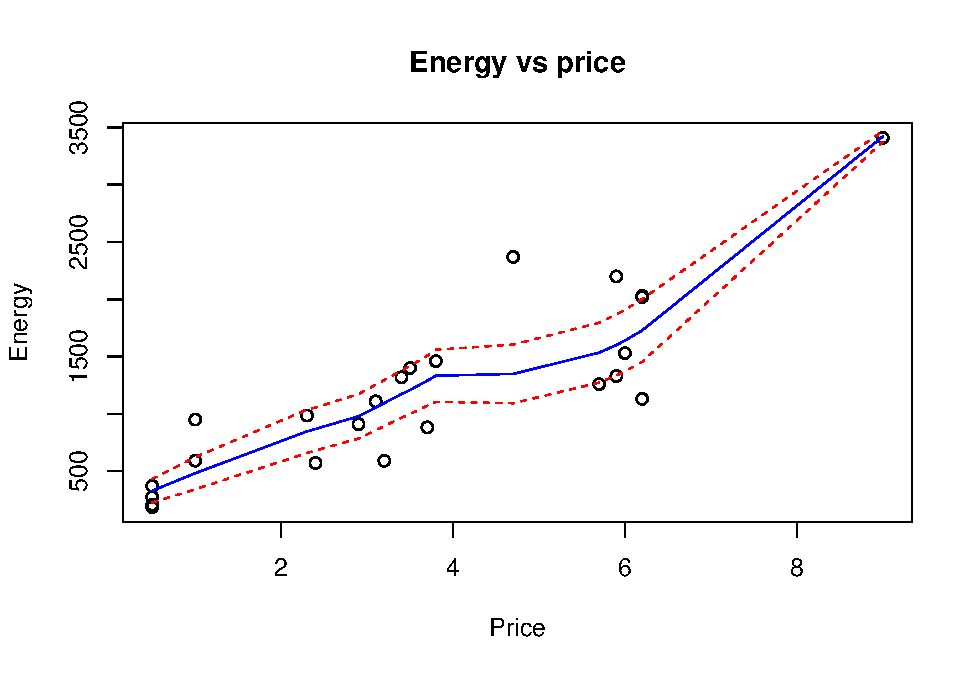
\includegraphics{Engsci211assignment2_task2_files/figure-latex/unnamed-chunk-2-1.pdf}

\hypertarget{original-eov-and-normality-checks}{%
\subparagraph{Original EOV and normality
checks}\label{original-eov-and-normality-checks}}

\begin{Shaded}
\begin{Highlighting}[]
\NormalTok{energy.fit =}\StringTok{ }\KeywordTok{lm}\NormalTok{(Energy}\OperatorTok{~}\NormalTok{Price, }\DataTypeTok{data =}\NormalTok{ energy.df)}
\KeywordTok{layout20x}\NormalTok{(}\DecValTok{1}\NormalTok{,}\DecValTok{2}\NormalTok{)}
\KeywordTok{plot}\NormalTok{(energy.fit,}\DataTypeTok{which=}\DecValTok{1}\NormalTok{)}
\KeywordTok{cooks20x}\NormalTok{(energy.fit)}
\end{Highlighting}
\end{Shaded}

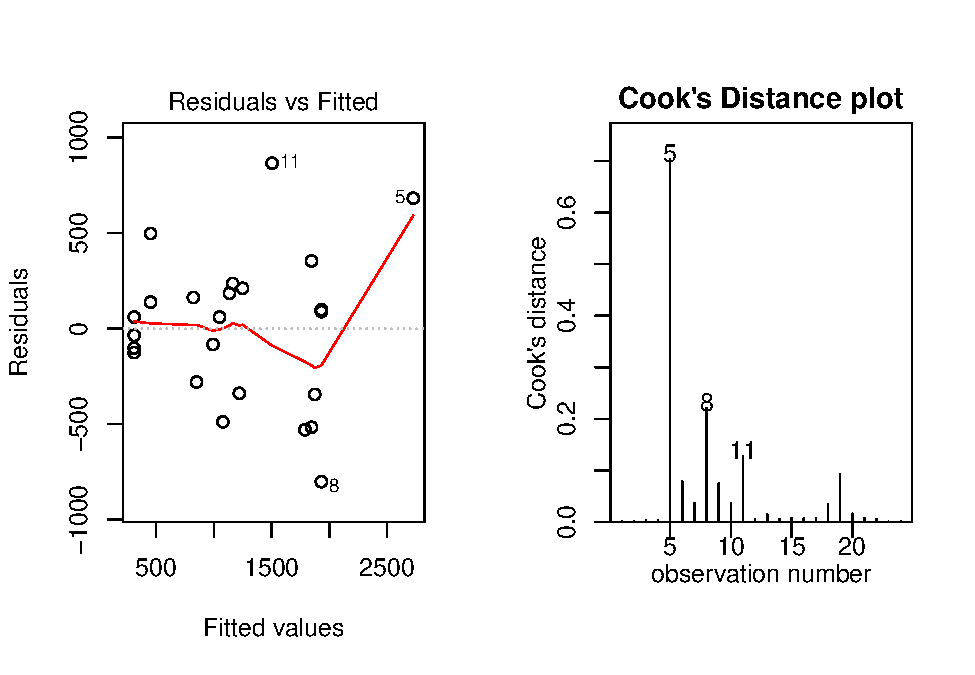
\includegraphics{Engsci211assignment2_task2_files/figure-latex/unnamed-chunk-3-1.pdf}

\begin{Shaded}
\begin{Highlighting}[]
\KeywordTok{summary}\NormalTok{(energy.fit)}
\end{Highlighting}
\end{Shaded}

\begin{verbatim}
## 
## Call:
## lm(formula = Energy ~ Price, data = energy.df)
## 
## Residuals:
##     Min      1Q  Median      3Q     Max 
## -801.23 -294.28   60.52  191.58  865.33 
## 
## Coefficients:
##             Estimate Std. Error t value Pr(>|t|)    
## (Intercept)   168.11     154.58   1.088    0.289    
## Price         284.37      35.67   7.973 6.24e-08 ***
## ---
## Signif. codes:  0 '***' 0.001 '**' 0.01 '*' 0.05 '.' 0.1 ' ' 1
## 
## Residual standard error: 402.5 on 22 degrees of freedom
## Multiple R-squared:  0.7429, Adjusted R-squared:  0.7312 
## F-statistic: 63.57 on 1 and 22 DF,  p-value: 6.245e-08
\end{verbatim}

\begin{Shaded}
\begin{Highlighting}[]
\KeywordTok{normcheck}\NormalTok{(energy.fit)}
\end{Highlighting}
\end{Shaded}

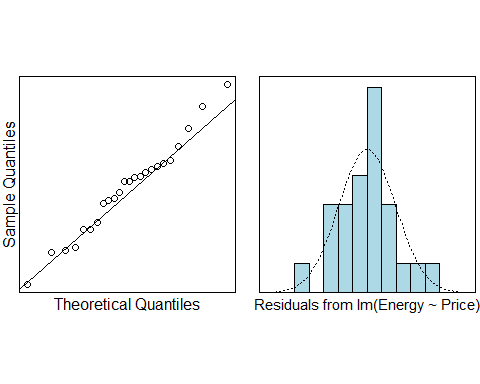
\includegraphics{Engsci211assignment2_task2_files/figure-latex/unnamed-chunk-3-2.pdf}
As we can see the data is quite heavily skewed, and, the observation at
position 5 is heavily influential with a cooks distance of 0.7, which is
greater than 0.4.

\begin{Shaded}
\begin{Highlighting}[]
\NormalTok{energy.fit2 <-}\StringTok{ }\KeywordTok{lm}\NormalTok{(Energy}\OperatorTok{~}\NormalTok{Price, }\DataTypeTok{data =}\NormalTok{ energy.df[}\OperatorTok{-}\DecValTok{5}\NormalTok{,])}
\KeywordTok{layout20x}\NormalTok{(}\DecValTok{1}\NormalTok{,}\DecValTok{2}\NormalTok{)}
\KeywordTok{plot}\NormalTok{(energy.fit2,}\DataTypeTok{which=}\DecValTok{1}\NormalTok{)}
\KeywordTok{cooks20x}\NormalTok{(energy.fit2)}
\end{Highlighting}
\end{Shaded}

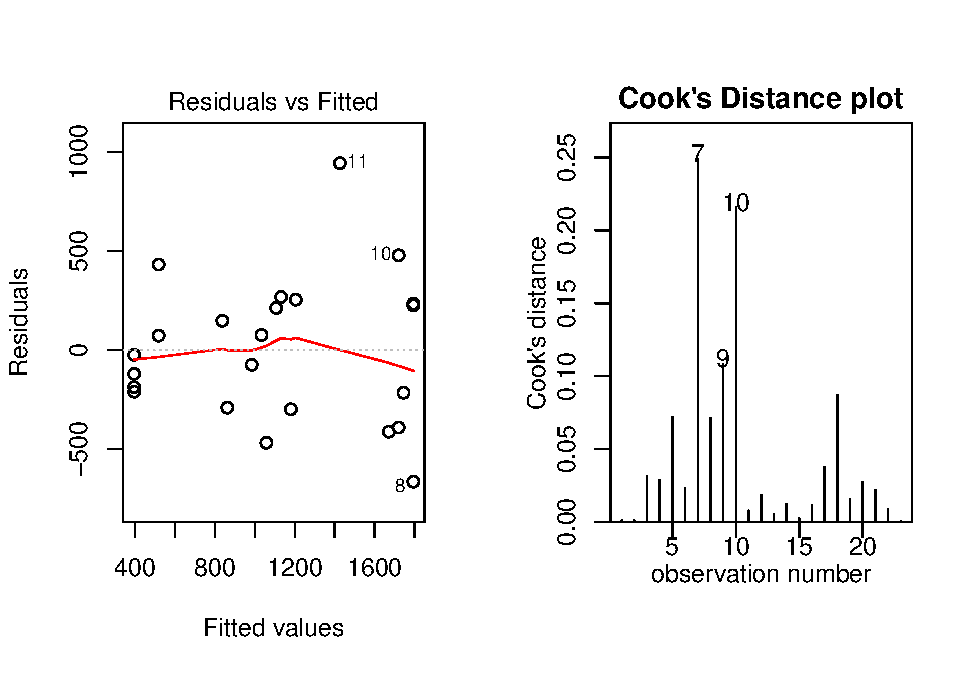
\includegraphics{Engsci211assignment2_task2_files/figure-latex/unnamed-chunk-4-1.pdf}

\begin{Shaded}
\begin{Highlighting}[]
\KeywordTok{summary}\NormalTok{(energy.fit2)}
\end{Highlighting}
\end{Shaded}

\begin{verbatim}
## 
## Call:
## lm(formula = Energy ~ Price, data = energy.df[-5, ])
## 
## Residuals:
##     Min      1Q  Median      3Q     Max 
## -664.34 -252.76  -23.76  230.66  943.97 
## 
## Coefficients:
##             Estimate Std. Error t value Pr(>|t|)    
## (Intercept)   271.99     151.53   1.795   0.0871 .  
## Price         245.54      37.79   6.497 1.95e-06 ***
## ---
## Signif. codes:  0 '***' 0.001 '**' 0.01 '*' 0.05 '.' 0.1 ' ' 1
## 
## Residual standard error: 373.6 on 21 degrees of freedom
## Multiple R-squared:  0.6678, Adjusted R-squared:  0.652 
## F-statistic: 42.21 on 1 and 21 DF,  p-value: 1.946e-06
\end{verbatim}

As we can see, the cooks distance plot no longer shows any influential
observations above 0.4. Similarly, we can see that by removing the
observation the estimate for price shifts from 284.37 to 245.54, which
is a change of 38.83, which is a change of more than 35.67, which is the
standard error, which implies observation 5 should be removed.

\begin{Shaded}
\begin{Highlighting}[]
\KeywordTok{trendscatter}\NormalTok{(Energy}\OperatorTok{~}\NormalTok{Price, }\DataTypeTok{data =}\NormalTok{ energy.df[}\OperatorTok{-}\DecValTok{5}\NormalTok{,])}
\end{Highlighting}
\end{Shaded}

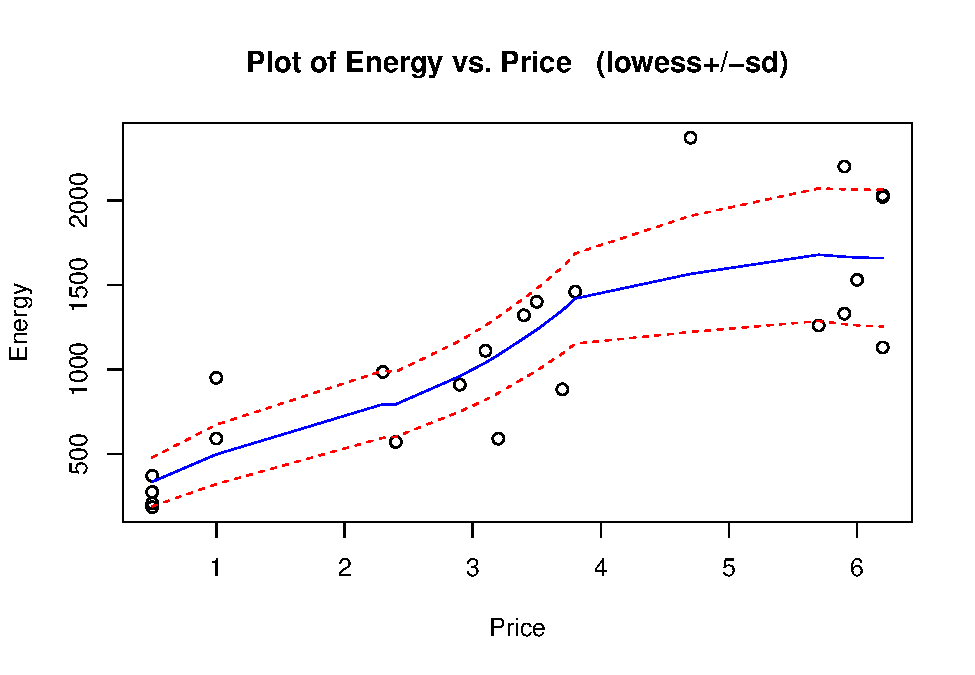
\includegraphics{Engsci211assignment2_task2_files/figure-latex/unnamed-chunk-5-1.pdf}

\begin{Shaded}
\begin{Highlighting}[]
\KeywordTok{normcheck}\NormalTok{(energy.fit2)}
\end{Highlighting}
\end{Shaded}

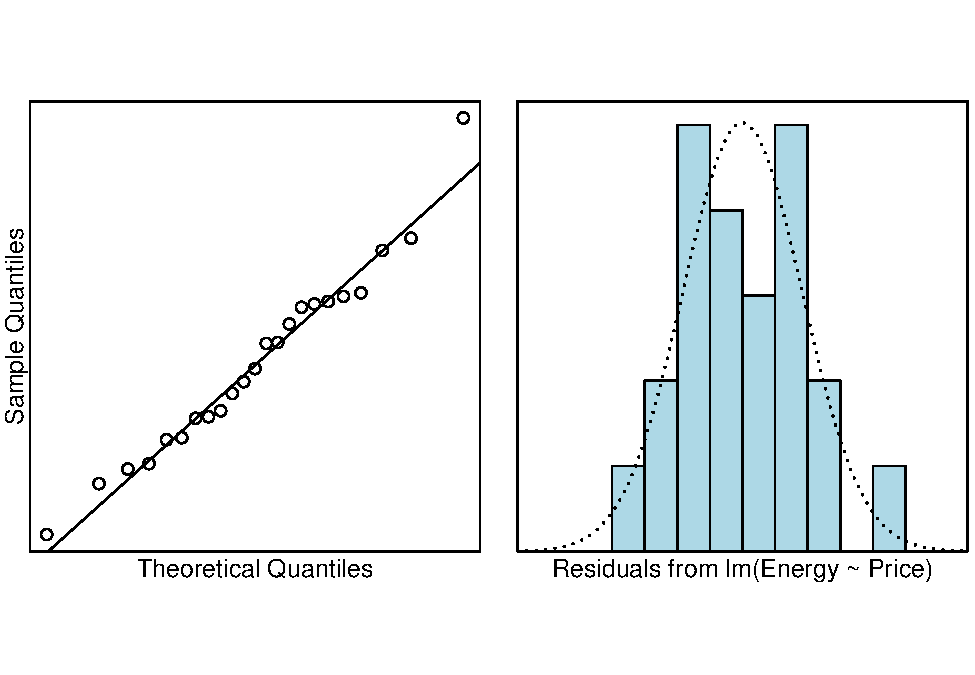
\includegraphics{Engsci211assignment2_task2_files/figure-latex/unnamed-chunk-6-1.pdf}
As we can see the sample with the influential observation removed, the
distribution is normal so our assumption of normality is correct.

\begin{Shaded}
\begin{Highlighting}[]
\KeywordTok{summary}\NormalTok{(energy.fit2)}
\end{Highlighting}
\end{Shaded}

\begin{verbatim}
## 
## Call:
## lm(formula = Energy ~ Price, data = energy.df[-5, ])
## 
## Residuals:
##     Min      1Q  Median      3Q     Max 
## -664.34 -252.76  -23.76  230.66  943.97 
## 
## Coefficients:
##             Estimate Std. Error t value Pr(>|t|)    
## (Intercept)   271.99     151.53   1.795   0.0871 .  
## Price         245.54      37.79   6.497 1.95e-06 ***
## ---
## Signif. codes:  0 '***' 0.001 '**' 0.01 '*' 0.05 '.' 0.1 ' ' 1
## 
## Residual standard error: 373.6 on 21 degrees of freedom
## Multiple R-squared:  0.6678, Adjusted R-squared:  0.652 
## F-statistic: 42.21 on 1 and 21 DF,  p-value: 1.946e-06
\end{verbatim}

\begin{Shaded}
\begin{Highlighting}[]
\NormalTok{pred.df =}\StringTok{ }\KeywordTok{data.frame}\NormalTok{(}\DataTypeTok{Price =} \FloatTok{5.90}\NormalTok{)}
\KeywordTok{predict}\NormalTok{(energy.fit2, pred.df, }\DataTypeTok{interval =} \StringTok{"prediction"}\NormalTok{)}
\end{Highlighting}
\end{Shaded}

\begin{verbatim}
##        fit      lwr      upr
## 1 1720.677 903.7747 2537.579
\end{verbatim}

\hypertarget{methods-and-assumption-checks}{%
\subsubsection{Methods and Assumption
Checks}\label{methods-and-assumption-checks}}

\hypertarget{executive-summary}{%
\subsubsection{Executive summary}\label{executive-summary}}


\end{document}
